\documentclass[reqno]{amsart}
\usepackage{graphicx}
\begin{document}

The pyrolysis model in Morvan and Dupuy 2004 is

\begin{equation}
  \frac{d}{dt}{\alpha \rho}=(\nu_{char}-\nu_{soot}-1)\dot{\omega}_{pyr}\,,
\label{eqn:Mdot}
\end{equation}
where $\alpha\rho$ is the mass and the pyrolysis model is 

\begin{equation}
  \dot{\omega}=\frac{Q}{\delta h} \frac{T-400}{100}\,.
\label{eqn:omdot}
\end{equation}
$Q$ is the heat received by the solid fuel, that is:

\begin{equation}
  \alpha \rho C \frac{dT}{dt}=Q\,.
\label{eqn:Tdot}
\end{equation}

The constant quantities are: $C$ specific heat of the material, $\delta h$ latent heat of pyrolysis $0.418\times 10^{6}$, $\nu{char,soot}$ the stoichometric coefficents of the reactions. 

Substituting equation \eqref{eqn:Tdot} and \eqref{eqn:omDot} into equation \eqref{eqn:Mdot} gives
\begin{equation}
  \frac{d}{dt}{\alpha \rho}=(\nu_{char}-\nu_{soot}-1)  \frac{\alpha \rho C}{\delta h}  \frac{T-400}{100} \frac{dT}{dt}\,.
\label{eqn:step1}
\end{equation}

Changing variables from $t$ to $T$ gives
\begin{equation}
  \frac{d}{dT}{\alpha \rho}=(\nu_{char}-\nu_{soot}-1)  \frac{\alpha \rho C}{\delta h}  \frac{T-400}{100}\,.
\label{eqn:step2}
\end{equation}

Then writing $M=\alpha \rho$ gives us an ode we can solve
\begin{align}
  \frac{d}{dT}{M}&=(\nu_{char}-\nu_{soot}-1)  \frac{M C}{\delta h}  \frac{T-400}{100}\,,\\
  M&=M(0) \exp(
\label{eqn:step2}
\end{align}

The other parameters are somewhat guessed. 
$C\approx 1900$ is guessed from data available on the internet. 
$\nu_{char}=8/3$ Poitere, Morvan, et al. 1998 
$\nu_{soot}=1$ because it gives a nice fit. 

\begin{figure}
\centering
  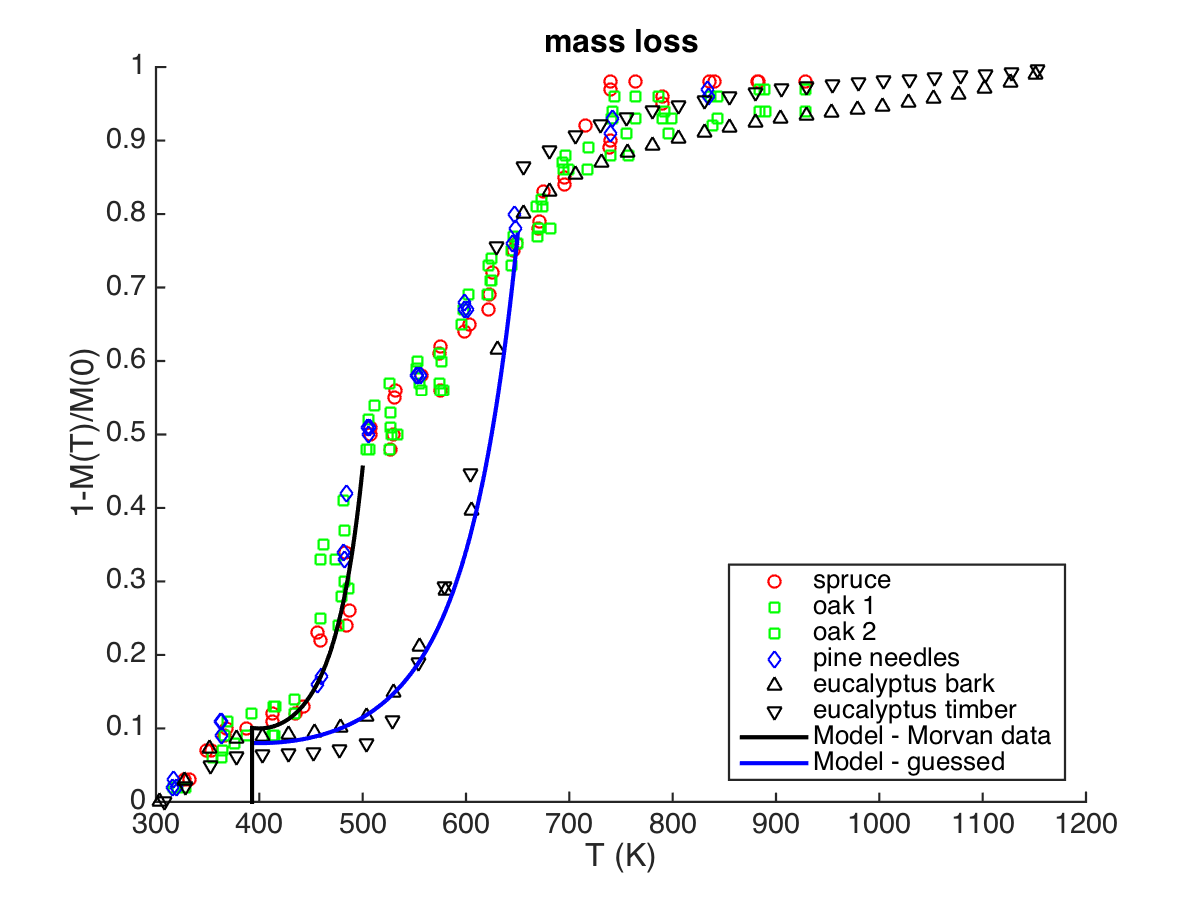
\includegraphics[scale=0.5]{massloss.png}
\caption{Dominique's and Rahul's TGA data with models}
\end{figure}
\end{document}
